\documentclass[sigconf]{acmart}
\setcopyright{none}
\settopmatter{printacmref=false,printccs=false,printfolios=true}
\renewcommand\footnotetextcopyrightpermission[1]{}
\acmConference[SymDiv Fall 2026]{SymDiv Advanced Topics in Program Analysis}{Fall 2026}{Singapore}
\acmYear{2026}
\copyrightyear{2026}
\usepackage{booktabs}
\usepackage{listings}
\usepackage{tikz}
\usetikzlibrary{arrows.meta,positioning}
\usepackage{xcolor}
\emergencystretch=3em
\raggedbottom
\lstset{language=C,basicstyle=\ttfamily\footnotesize,columns=fullflexible,keepspaces=true,breaklines=true,frame=single,showstringspaces=false}
\newcommand{\AbstractResultsVThree}{Under the primary 128-state budget, guidance confirms 9/9 diagnostic defects, versus 5/9 for DFS and 7/9 CSA warnings. The unverified model makes 1 false positive; guided verification accepts none. The new Juliet stratum remains at 4/4 positives for both guided and plain symbolic search. Charging observed model latency to a 20-second serial replay reverses the diagnostic comparison: DFS confirms 9/9, guidance 8/9.}
\newcommand{\ResourceResultsVThree}{Table~\ref{tab:v3-primary} shows a measurable contribution from changing the model's role. Guidance confirms all nine diagnostic positives, while DFS and the static heuristic each confirm five; the three random orders confirm five, five, and six. Across all nine positive files, including capped misses, guidance spends 270 state pops compared with DFS's 860. This is not a matched-success speedup ratio: the DFS total includes four exhausted searches. CSA finds seven positives and misses the depth-five and depth-seven loops. All verified systems have zero false positives. Guided search completely refutes three diagnostic negatives and leaves six unknown; those six contribute warning TNs but are not safety proofs. LLM-only finds all nine positives but makes one false-positive claim. On the new Juliet files, every custom search order finds four positives and refutes four negatives at the primary budget; CSA finds the two fixed-zero positives and does not warn on the two random-source positives. The external stratum therefore shows no additional discovery from neural ordering.}
\newcommand{\SensitivityResultsVThree}{At 64 states, guided discovery is 8/9 compared with DFS's 2/9 and a range of two to three for the random orders. At 512 states, guidance remains 9/9, DFS rises to 8/9, and random seed 47 also reaches nine. Thus the advantage narrows as ordinary search receives more work. Table~\ref{tab:v3-budgets} retains every seed and budget.}
\newcommand{\FeedbackResultsVThree}{The primary feedback arm triggers 0 correction requests and has the same predictions and state counts as guidance alone. This is a real limitation of its trigger, not evidence that feedback is unnecessary in general. In the natural false-positive case d005, the 48-pop probe ends before a failed denominator query is available. Later failures therefore reach DFS fallback rather than the model. A trigger tied to the first failed candidate, subject to a remaining-budget threshold, is a concrete next revision. It was not retroactively substituted into this frozen run. In a separate six-branch diagnostic, deliberately injected all-true advice produces an actual failed probe. One genuine model correction leads to a witness after 57 total pops and 62 solver calls, versus 109 pops and 129 calls with DFS fallback alone. Both variants eventually succeed, and the correction costs 10.73\,s. Both resulting witnesses are confirmed in compiled C. This demonstrates recovery and a search reduction, not a naturally observed primary repair or an end-to-end speedup.}
\newcommand{\LatencyResultsVThree}{The 26 primary requests consume 479,894 reported tokens and 325.71\,s of service time (median 11.30\,s per request). The separate development smoke uses 18,129 tokens, and the injected-feedback call uses 19,755; neither is pooled into primary counts. In the 20\,s latency-accounted comparison, all traditional custom orders find nine diagnostic positives and refute nine negatives. Guidance finds eight positives, refutes eight negatives, and returns two unknowns. The recorded request for d001 already exceeds 20\,s, leaving no local search time. For safe d015, about 2.1\,s remain after the request; primary search exhausts that time just before complete refutation. During offline reproduction, its two guided arms finish in that allowance and return complete refutation instead. Their warning predictions stay negative. This recorded disposition change illustrates timing sensitivity, and is retained rather than rerunning until the original status reappears. The external Juliet predictions remain unchanged. Across all 26 files, DFS's local wall-regime search totals 18.42\,s; individual files, rather than that sum, receive the 20\,s allowance. Table~\ref{tab:v3-cost} separates observed model latency from local resource-run costs.}
\newcommand{\CaseResultsVThree}{In d007, seven independent conditions update a weighted sum. The real branch IDs let the model prioritize a feasible zero-denominator vector; guided search finds it in 17 pops, while DFS reaches its 128-pop limit without a witness. In the depth-seven loop d016, the 48-pop advice phase ends before the sink. Its retained frontier and DFS fallback still find a witness at pop 104. The result therefore depends on guidance plus retained alternatives, not on following a complete neural path. The natural model error is more revealing: d005 has denominator $2d-11$, which cannot be zero for integral $d$. The model assigns confidence 1.0 and claims that $d=5$ makes $2\times5-11=0$; the actual value is $-1$. The source query rejects tested zero-denominator paths. At 128 pops the overall file remains unknown, so the method withholds the false warning without claiming a complete proof. With the larger wall-regime exploration it returns a complete refutation. This is an observed verification benefit distinct from the intentionally injected robustness example.}
\newcommand{\WitnessResultsVThree}{The primary search arms emit 304 accepted-result occurrences across systems and budgets. Deduplication by case, site, and complete input assignment yields 25 distinct witnesses, all 25 confirmed by UBSan at the expected line. These cover all 13 positive files. Duplicated appearances are not counted as new bugs.}
\newcommand{\RealWorldScreenVThree}{Three pinned upstream releases were screened using one fixed translation unit each: libpng 1.6.44 (8 sink-containing functions, 23 integer arithmetic sites), libsndfile 1.2.2 (59 sink-containing functions, 59 integer arithmetic sites), libtiff 4.7.0 (10 sink-containing functions, 31 integer arithmetic sites). CMake configuration and each selected unit's Clang syntax/AST compilation succeeded with recorded build flags. An initial libpng attempt failed because its generated configuration header was absent; executing upstream's header-generation target resolved that build-context issue, and the failed attempt is retained. This is not a complete library build or a whole-project coverage measurement. Every sink-containing function in these selected units requires at least one unsupported structural feature, including memory access, non-scalar types, or calls needing reviewed summaries. The direct restricted frontend also rejects their preprocessing directives. No function was manually sliced to remove those requirements, no model was asked to invent a library summary, and no bug-recall score is assigned. Exact commits, archive/source hashes, compile commands, per-function blockers, and diagnostics are recorded in the artifact.}
\newcommand{\ValidationResultsVThree}{The full regression suite passes 82 tests. The new scheduler and guidance checks extend the original 62-test suite, and a separate run preserves all 48 historical warning classifications. The accepted primary and injected witnesses were rechecked with the native compiler.}
\newcommand{\ReproductionResultsVThree}{The completed offline reproduction makes zero model calls, regenerates all 26 new source files identically, and matches every system's prediction and disposition in the primary, 64-state, and 512-state resource regimes. All wall-regime warning predictions also match; two timed dispositions change from unknown to complete refutation on safe d015. V2's two strata also retain their earlier metrics and dispositions. Local setup and exact commands are in both the repository-root and project READMEs.}
\newcommand{\PublicationStatusVThree}{This delivery is a local artifact. No public repository URL has been supplied or published for it, so the course's public-artifact requirement remains open. The report intentionally does not present a placeholder as a working link. Publication, anonymous-access verification, student review of the AI disclosure, and Canvas submission remain the final delivery actions.}
\newcommand{\ConclusionResultsVThree}{On controlled resource-sensitive programs, the change increases confirmed diagnostic discovery from DFS's five to nine positives under the primary cap and withholds a genuine model false positive. On the new external Juliet stratum it adds no discoveries. Observed service latency reverses the diagnostic comparison under the 20\,s accounting rule. The frozen feedback trigger has no primary effect, while a separate injected-error experiment confirms that real feedback can reduce subsequent search. These findings support a bounded role for neural priority advice and expose concrete limits in timing, feedback activation, and real-source semantics.}

\title[SymDiv: Source-Verified Neural Path Guidance]{SymDiv: Source-Verified Neural Path Guidance under Search and Latency Budgets}
\author{SymDiv Project}


\begin{document}
\begin{abstract}
A language model can propose a plausible bug without describing a feasible
program execution. This project explores where neural advice should enter
a static analyzer for integer division and remainder by zero in C. An initial
predicate-only verifier could accept invented executions. A second version
repaired the source semantics, but full path construction before neural
filtering left little opportunity for the model to help. The third version
instead uses model-selected branch directions to prioritize a resumable
symbolic worklist. Every accepted witness satisfies constraints derived from
the source; advice never changes program semantics or deletes an alternative.
We compare Clang Static Analyzer, unverified model predictions, DFS, a cheap
static heuristic, three random orders, and guidance with and without one
verification-feedback correction. The new evaluation separates 18 authored
mechanism diagnostics from eight mechanically derived Juliet subjects and
retains 48 historical subjects as regressions.
\AbstractResultsVThree{}
The study distinguishes search efficiency from service latency, records
failed and inconclusive paths, and validates accepted inputs in compiled C.
\end{abstract}
\maketitle

\section{Introduction}
Static analysis needs a defensible connection between a warning and the
program that produced it. In a neural--symbolic analyzer, an SMT solver can
establish that a model's explanation is satisfiable while the explanation
omits the very guard that makes the program safe. At the other extreme,
a symbolic engine can already do all the necessary reasoning, leaving the
language model as an expensive filter after the work is complete. These are
different design failures: an unsound acceptance boundary and an ineffective
division of labor.

SymDiv studies both failures on the same concrete problem: whether an integer
division or remainder can execute with a zero denominator. The traditional
external baseline is Clang Static Analyzer (CSA), an executable path-sensitive
static analyzer with the \texttt{core.DivideZero} checker
\cite{clang-checkers,clang-cli}. The proposed solution is a small,
independently implemented symbolic interpreter around Clang's parser and Z3.
The project does not adopt an existing neural static-analysis tool as its
main solution. Codex CLI supplies authenticated model requests and structured
output; it does not implement the analysis method.

The project evolved through three versions. Version 1 accepted
model-supplied predicates without validating their correspondence to the
source. Version 2 introduced source-derived control flow, assignments,
integer semantics, and explicit incompleteness. On 48 small subjects,
its hybrid and symbolic-only variants had identical warning classifications.
That finding motivated an architectural change instead of a more favorable
description of the same result. Version 3 moves the model before path
exploration: the model recommends branch decisions, and the interpreter
uses those decisions only to order a retained frontier.

The resulting research questions are:
\begin{enumerate}
\item Under identical state and solver-call budgets, does neural guidance
discover more source-confirmed defects than inexpensive search orders?
\item Does one correction from actual verifier feedback improve discovery,
and what happens when advice is incorrect or incomplete?
\item Does any search advantage survive accounting for model latency, and
how far does the supported semantics extend beyond diagnostic programs?
\end{enumerate}
The contribution is an inspectable experimental method and its evidence,
not a claim to invent neural path prioritization or to outperform
general-purpose analyzers on production code. An improvement in bounded
discovery and an increase in total latency can both be true.

\section{Problem and Traditional Baseline}
\subsection{Analysis contract}
For a function-entry input $x$, let $\pi$ be a path to an integer arithmetic
site $s$, let $C_\pi(x)$ include branch conditions and definedness guards,
and let $d_s(x)$ be the denominator computed along that path. A confirmed
finding requires
\[
  \exists x,\pi:\ C_\pi(x)\ \land\ d_s(x)=0.
\]
The numerator and earlier operations must be evaluated consistently with
the declared source model. An earlier division by zero or signed overflow
cannot be used to justify a later warning. The tool emits at most one
confirmed finding per file in v3 because the evaluation asks whether any
integer zero-denominator defect exists.

The interpreter supports scalar 32-bit \texttt{int} and \texttt{unsigned int},
local assignments, lexical shadowing, integer comparisons and arithmetic,
short-circuit and conditional expressions, \texttt{if}, bounded
\texttt{for}/\texttt{while}/\texttt{do} loops, and return/break/continue.
Signed division truncates toward zero; signed remainder has the dividend's
sign. Unsigned arithmetic wraps modulo $2^{32}$. Signed overflow paths are
excluded and the \texttt{INT\_MIN/-1} continuation is guarded, following
the relevant C rules and the recorded target assumptions \cite{c11}.
The model's prose cannot change any of these operations.

External \texttt{rand()} results are independent symbolic integers in
$[0,2^{31}-1]$. This is an explicit environment abstraction, not a model of
a particular seeded pseudorandom generator. The declared void printing
functions are observational. Arbitrary calls, pointer memory, mutable
globals, unsupported integer types, and uninitialized reads cause
incompleteness. Each function containing a sink is analyzed from its entry;
we do not claim whole-program calling-context feasibility.

The result categories separate an existential witness, complete refutation
within the supported model, and unknown. A reachable continuation beyond
eight loop iterations, a final solver timeout, an unsupported operation,
or exhausted resources produces unknown unless another path has already
provided a witness. Warning-based true negatives therefore do not necessarily
mean safety was established.

\subsection{CSA as the external comparator}
CSA explores a graph of symbolic program states and reports suspicious
operations using checkers. We invoke its command-line analyzer on the exact
same derived C files with \texttt{core.DivideZero}, C11, and SARIF output.
Commands, diagnostics, compiler version, completion status, and runtime are
recorded. A successful process and readable analyzer report are required;
a crash or missing report is not scored as a negative.

CSA's warning policy differs from the existential input contract. For
example, a possibly zero unconstrained parameter or random result need not
receive the same warning as a definitely zero value. A missed warning under
our label policy is still a false negative in our table, but it is not
automatically a neural reasoning victory. The same-engine DFS, heuristic,
and random controls are essential for separating the value of search advice
from the value of the custom symbolic semantics.

\section{Design Iterations}
\subsection{Why satisfiable advice was insufficient}
Consider \texttt{if(x==0) return 0; return 42/x;}. The v1 formula could accept
$x=0$ if the model omitted the early return. A similar defect allowed a
local \texttt{d=7} to become an unconstrained symbolic variable. These are
source-translation failures, even if the model happens to classify the
primary dataset correctly. Regressions deliberately inject such wrong
hypotheses; they are not counted as naturally occurring model mistakes.

V2 repaired this boundary by constructing source-feasible states before
checking model predicates. However, if $H$ is the model's additional
predicate and $S=C_\pi\land d_s=0$, then
$\mathrm{models}(S\land H)\subseteq\mathrm{models}(S)$.
With complete exploration and successful solving, additional predicates
cannot create new real defects. They can restrict useful candidates or,
under limited solving time, change solver difficulty. V2 did not measure
a benefit from the latter effect, and its eager path construction could
not be accelerated by a suggestion received afterward.

The historical 24-case pilot and 24-case Juliet run are preserved unchanged.
Each has 12 positives; CSA finds nine and six respectively, while LLM-only,
v2 hybrid, and symbolic-only each find all 12 with no false positives.
The symbolic-only pilot includes two negative abstentions. All 24 accepted
hybrid witnesses were confirmed in compiled C. These results motivate v3;
they are not reused as previously unseen evidence for the new design.

\subsection{V3: advice orders a worklist}
Clang creates a JSON AST. The frontend assigns each branch a stable identifier
from the source hash, function, source offset, and branch kind. A model receives
the complete source, division sites, and a branch catalog, without labels,
baseline predictions, or files from the artifact. Structured output includes
a verdict for each site and a list of
\texttt{(branch\_id, visit, take)} preferences. Visit identifies an occurrence
inside a loop; take selects the true/body or false/exit direction.
Malformed identifiers, duplicates, and non-Boolean choices are rejected.
The old predicate field must be empty.

A search state contains the symbolic store, lexical bindings, source
constraints, inputs, decision trace, and continuation frames. Executing an
\texttt{if} queues both successors. Loop frames also retain the exit
alternative and the iteration count. A heap orders states by the number of
disagreements between their trace and supplied preferences, breaking ties
by the most recently queued state. Unspecified decisions tie. Advice never
substitutes for evaluating the actual condition.

\begin{figure}[t]
\centering
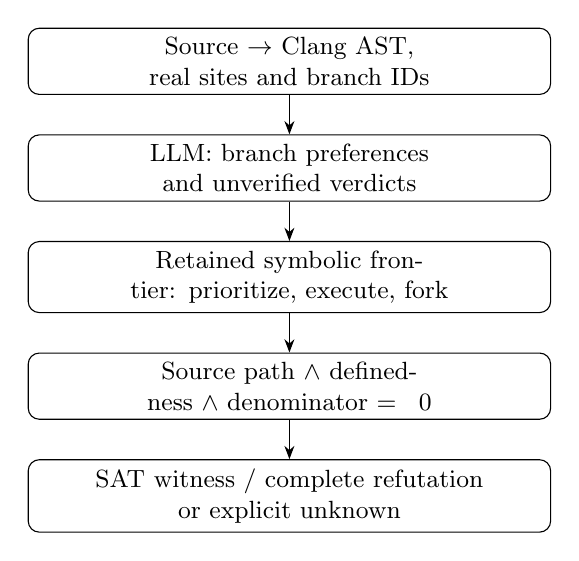
\begin{tikzpicture}[node distance=5mm,font=\small,
 box/.style={draw,rounded corners,align=center,text width=6.4cm,minimum height=7mm},
 >=Stealth]
\node[box] (ast) {Source $\rightarrow$ Clang AST, real sites and branch IDs};
\node[box,below=of ast] (llm) {LLM: branch preferences and unverified verdicts};
\node[box,below=of llm] (queue) {Retained symbolic frontier: prioritize, execute, fork};
\node[box,below=of queue] (check) {Source path $\land$ definedness $\land$ denominator $=0$};
\node[box,below=of check] (end) {SAT witness / complete refutation\\or explicit unknown};
\draw[->] (ast)--(llm);\draw[->] (llm)--(queue);
\draw[->] (queue)--(check);\draw[->] (check)--(end);
\end{tikzpicture}
\caption{V3's acceptance formula comes only from the program. Feedback can
reorder the remaining frontier once; DFS uses any remaining budget.}
\label{fig:workflow}
\end{figure}

When a sink is reached, the interpreter checks its denominator for zero
under the accumulated constraints. A fixed, small set of concrete input
vectors first attempts exact substitution; it can find a witness but never
prove safety. Otherwise Z3 checks the formula. The same seed attempts and
solver are available to every search control. A feasibility-pruning timeout
retains the path; only a definitive UNSAT result prunes it. A final
zero-denominator query that times out records unknown.

\subsection{Correction and fallback}
The first guided phase spends at most 48 state pops. If there is no witness,
the frontier remains nonempty, the model proposed bug or unknown, and an
actual failed source check is available, the feedback variant may make
one correction request. Feedback contains the attempted trace, actual
UNSAT core for a zero-denominator query when available, source failures,
and spent-resource counts. It contains no benchmark label or preferred
baseline answer. A failed pruning query is described as an unreachable
branch; the implementation does not invent an UNSAT core for it.

Corrected preferences reprioritize the existing heap for at most another
48 state pops. The no-feedback variant, or either variant after its guided
phase, uses DFS on the retained frontier with the remaining budget.
Counters do not reset, discarded alternatives are not recreated, and a
repair receives no free full-budget restart. A model-safe verdict never
suppresses symbolic search. Thus an incorrect suggestion can waste
resources, but cannot directly create an accepted execution.

This interface is deliberately modest. It has no learned invariant
generation, interprocedural summaries, or neural memory model. Those
extensions would require new correctness boundaries and identical semantic
support for the traditional controls. The present experiment isolates
priority advice and one bounded correction.

\section{Experimental Design}
\subsection{Separate evidence roles}
The v3 cohort is frozen before the first primary model prediction, including
source and configuration hashes, prompt, schema, implementation, and case
order. A separate three-branch development smoke call establishes that the
interface works and exposes the magnitude of model latency. The 48 earlier
subjects are regression data; all preserve their warning classifications
under the new execution engine.

\textbf{Authored diagnostics (18 files).} Three families each contain
depths 3, 5, and 7, with one positive and one safe paired file.
Independent inputs, correlated bits of a bounded integer, or independent
random values in a bounded loop choose additions and subtractions of
powers of two. A positive denominator is $d-t$ for a fixed attainable
target $t$; its safe mate is $2d-(2t+1)$, which is always odd. The complete
finite set of $2^k$ branch vectors is enumerated to check these labels.
Values are small enough to avoid overflow. This creates controlled path
growth and numerical relationships, including repeated branch decisions,
without claiming that the patterns represent production programs.

The generator fixes target decisions by an index rule before any model
result. It saves label evidence separately from model input. These samples
were authored and inspected during development: freezing them makes the
experiment auditable, but does not make them independent or unseen
development data. The diagnostic claim is causal and narrow: changing
priority can matter when exploration is constrained.

\textbf{New external Juliet stratum (eight files).} The official NIST
Juliet 1.3 archive provides independent source authorship \cite{juliet}.
We select previously unused control-flow variants 02 (literal
conditions, division) and 04 (constant-global conditions, remainder),
with both zero and random source families and both bad and complete good
branches. These eight derived files contain 20 arithmetic sites.
The transformation reuses the audited v2 materializer: Clang preprocessing,
the exact upstream random macros, neutralized label-bearing identifiers,
and neutralized diagnostic strings. All good helper functions remain.
The artifact retains raw source bytes, checksums, flags, and mappings.

This selection extends flow-family coverage within the supported scalar
subset. It is not a random sample of Juliet, a new corpus family, or a
guarantee against model training exposure. Mutable-global, pointer,
arbitrary-call, switch, and goto patterns remain outside the implementation.
The external stratum is reported separately so a favorable diagnostic
result cannot be disguised as a production or independent-benchmark gain.

\subsection{Systems and budgets}
The same-engine controls are true-first DFS, a fixed syntactic heuristic,
and random heap priorities with seeds 11, 29, and 47. The heuristic prefers
an arm containing a division/remainder, then a literal zero assignment to
a simple denominator variable; ties prefer true. It is inexpensive and
documented, not an oracle for the diagnostic arithmetic. All three random
runs are shown; none is chosen after observing results.

The neural arms are LLM-only (any initial bug verdict), guidance without
feedback, and guidance with the one-correction policy. They share the same
first recorded response per subject. This paired design isolates the
verification/search policy from variation between independent first calls.
Only a qualifying feedback request consumes an additional call.
The model is \texttt{gpt-5.6-sol} with medium reasoning effort through
source-only Codex CLI requests. Tool use in a model response invalidates
the protocol. No response contains the expected labels.

The primary mechanical budget is 128 worklist pops and 256 solver calls,
with eight loop iterations, a 1,000\,ms final-query cap, a 25\,ms pruning
cap, and a 20\,s local-search ceiling. A pop can process a source statement
or a continuation/scope frame, so it is an implementation unit, not a
claim of equivalence to a KLEE instruction or a CSA node. The seed batch
count is recorded separately. Every search order receives the same
semantics, state definition, solver, and limits. Sensitivity runs use
64/128 and 512/1,024 state/query caps with the same recorded responses;
they do not retune the prompt.

The model budget is 40 calls, 900,000 reported input-plus-output tokens,
90 seconds per request, and no retries. Calls stop on an unavailable usage
record or error. A completed call that crosses the token cap is retained
and prevents further requests. Missing cases cannot be scored as negatives.
These ceilings were fixed before primary predictions. Model tokens are
CLI-reported usage, including harness context; they are not just the number
of C-source tokens and are not converted to an assumed monetary price.

\subsection{Latency accounting and outcome validation}
To examine a practical budget, we also execute local searches with a
20\,s deadline, charging AST preparation plus the recorded first-call
latency before neural search starts. A used repair consumes its recorded
latency from the same deadline. Traditional controls receive the full
remaining local time and very large state/query caps. If a model call
already exceeds 20\,s, that neural arm has no search time.

This is explicitly a \emph{serial latency-accounted replay}, not an
independent live deadline experiment. It asks what these particular
recorded responses and latencies permit when combined with measured local
search. It excludes parallel speculative DFS during a request and does
not estimate future service latency. Reporting this construction is
preferable to silently omitting the model wait or treating an offline
replay as a free model.

We report warning TP/FP/TN/FN, recall, complete refutations, unknowns,
worklist pops, solver calls, first-witness timing, service latency,
model calls, and tokens. Unknown on a positive is a warning false negative;
unknown on a negative remains unknown even if it contributes a TN.
The scorer rejects incomplete cohorts, duplicated IDs, mismatched source
hashes, and non-Boolean predictions. Checkpoints retain every actual
response and failure.

Accepted source witnesses are replayed in C compiled with Clang's
undefined-behavior sanitizer, with optimization and error recovery disabled.
The exact flags are retained in the artifact. The diagnostic
must identify division by zero at the recorded source line. Harnesses call
the analyzed entry and supply its scalar parameters and recorded
\texttt{rand()} stream. Symbolic values allocated in an inactive
short-circuit or conditional arm are excluded from that stream. Dynamic
execution checks evidence; it is not the detection method.

\section{Results and Interpretation}
\begin{table*}[t]\centering\small
\caption{Primary 128-state/256-query comparison. Each stratum is balanced: diagnostic 9 positive/9 negative, Juliet 4/4. U is explicit unknown. TN is 9-FP or 4-FP; U is not a safety proof. CSA and LLM-only use their native classification behavior, not the custom state cap.}\label{tab:v3-primary}
\begin{tabular}{lrrrrrrrr}\toprule
&\multicolumn{4}{c}{Authored diagnostics (18)}&\multicolumn{4}{c}{New Juliet flows (8)}\\
System & TP & FP & FN & U & TP & FP & FN & U\\\midrule
Clang CSA & 7 & 0 & 2 & 0 & 2 & 0 & 2 & 0\\
DFS & 5 & 0 & 4 & 10 & 4 & 0 & 0 & 0\\
Static heuristic & 5 & 0 & 4 & 10 & 4 & 0 & 0 & 0\\
Random 11 & 5 & 0 & 4 & 10 & 4 & 0 & 0 & 0\\
Random 29 & 5 & 0 & 4 & 10 & 4 & 0 & 0 & 0\\
Random 47 & 6 & 0 & 3 & 9 & 4 & 0 & 0 & 0\\
LLM-only & 9 & 1 & 0 & 0 & 4 & 0 & 0 & 0\\
Guided & 9 & 0 & 0 & 6 & 4 & 0 & 0 & 0\\
Guided + feedback & 9 & 0 & 0 & 6 & 4 & 0 & 0 & 0\\
\bottomrule\end{tabular}\end{table*}
\begin{table}[t]\centering\small
\caption{Confirmed diagnostic positives (out of 9) across budgets. All listed search systems have zero false positives. Wall column includes recorded model latency.}\label{tab:v3-budgets}
\begin{tabular}{lrrrr}\toprule System&64 states&128&512&20\,s\\\midrule
DFS & 2 & 5 & 8 & 9\\
Static heuristic & 2 & 5 & 8 & 9\\
Random 11 & 2 & 5 & 8 & 9\\
Random 29 & 3 & 5 & 8 & 9\\
Random 47 & 3 & 6 & 9 & 9\\
Guided & 8 & 9 & 9 & 8\\
Guided + feedback & 8 & 9 & 9 & 8\\
\bottomrule\end{tabular}\end{table}
\begin{table}[t]\centering\small
\caption{Observed cost over all 26 files in the resource regime. Neural arms share first responses; their service costs must not be added as separate actual calls. Local excludes AST preparation.}\label{tab:v3-cost}
\begin{tabular}{lrrr}\toprule System&State pops&Local (s)&Model (s)\\\midrule
Clang CSA & -- & 0.47 & --\\
DFS & 2131 & 4.93 & --\\
Static heuristic & 2154 & 4.51 & --\\
Random 11 & 2160 & 4.34 & --\\
Random 29 & 2115 & 4.48 & --\\
Random 47 & 2074 & 4.14 & --\\
Guided & 1541 & 3.45 & 325.71\\
Guided + feedback & 1541 & 3.32 & 325.71\\
\bottomrule\end{tabular}\end{table}

\subsection{Discovery under a fixed exploration budget}
\ResourceResultsVThree{}
The two strata answer different questions. The diagnostic cohort tests
whether the placement of the neural component changes an observable
search decision under scarcity. The external cohort tests that the same
interface works on separately authored retained transformations. Neither
justifies combining all files into a single headline production accuracy.

\SensitivityResultsVThree{}
Budget sensitivity matters because a search order can appear superior
when the limit cuts off another order just before its witness. The
reported settings are therefore points on a resource curve, rather than
a claim that one fixed state cap is intrinsically representative.
The safe mates are also informative: prioritizing a witness does not
usually avoid the work needed to refute every path.

\subsection{What feedback actually contributed}
\FeedbackResultsVThree{}
The feedback mechanism is evaluated as implemented, including absent
triggers and ineffective corrections. A naturally correct first proposal
is not evidence that feedback repaired it. Injected wrong advice is
reported separately as a robustness test. Its purpose is to verify that
source constraints reject an impossible path and the remaining frontier
can still be explored, not to inflate the primary error-correction count.

\subsection{Latency can reverse the practical conclusion}
\LatencyResultsVThree{}
The mechanism and deployment questions should not be conflated. Reducing
state expansion is useful evidence about guidance, but a local analyzer
may finish before a remote model responds. Conversely, the current tiny
programs do not establish how the tradeoff would behave when ordinary
search runs for minutes. A longer-workload claim would require suitable
independent subjects, stronger traditional heuristics, and new timing
experiments; it cannot be inferred from a positive state-budget result.

\subsection{Representative traces and failures}
\CaseResultsVThree{}
The recorded trace is an explanation of the actual source execution,
rather than a restatement of the neural rationale. This distinction lets
the reader inspect which branch choices were useful, whether a suggested
decision was encountered at all, and where fallback consumed the remaining
budget. Retaining raw failed checks also prevents a successful final
witness from concealing an initially incorrect proposal.

\WitnessResultsVThree{}

\section{Applicability and Correctness}
\subsection{A small real-source feasibility screen}
\RealWorldScreenVThree{}
The upstream source repositories are documented by their maintainers
\cite{libpng,libsndfile,libtiff}; the artifact pins exact commits.
This screen measures the implementation boundary, not vulnerability
discovery. It does not assign ground-truth bug labels to a library merely
because no warning was emitted, and it does not extract arithmetic while
discarding the pointer and calling context needed to interpret it. The
negative applicability result motivates a future memory/call model or a
different backend; it is not repaired by asking the model to declare
unsupported code safe.

\subsection{Regression and robustness evidence}
\ValidationResultsVThree{}
The tests target defects that could invalidate accepted evidence:
scope restoration across loops and nested blocks, loop increment after
continue, break in nested loops, signed overflow exclusion, unsigned
wraparound, earlier arithmetic undefinedness, conditional evaluation,
unsupported calls, malformed suggestions, and source-location stability
after checkout relocation.

The frontier tests check a different invariant from the arithmetic tests.
Reprioritization preserves queued task identities and spent counters;
fallback uses those same tasks. The budget tests require unknown when
time, states, or solver calls are exhausted. A separate executable
regression chooses the false arm of a conditional containing \texttt{rand()},
ensuring that inactive symbolic inputs do not shift the concrete random
stream. These checks increase confidence in the implementation without
constituting a proof of the entire interpreter.

\section{Related Work and Validity Limits}
Z3 supplies SMT solving, not a C frontend \cite{z3}. CSA supplies the
independent external static-analysis baseline; sharing Clang's parsing
infrastructure does not mean SymDiv reuses CSA warnings or symbolic states.
The same-engine controls intentionally share more implementation so that
they isolate the priority policy.

AutoBug decomposes LLM analysis into path-oriented subtasks represented in
code, allowing the model to perform approximate symbolic reasoning
\cite{autobug}. SymDiv instead keeps source execution in a restricted
interpreter and limits the model to suggestions whose consequences must
pass that interpreter. KLEECopilot uses model-marked vulnerable regions
and loop-aware prioritization in KLEE \cite{kleecopilot}. The high-level
idea of neural search guidance is therefore prior work, not a novelty claim
of this project. SymDiv's concrete interface is an occurrence-indexed
branch preference list, with one source-feedback correction and retained
frontier accounting. No code or prebuilt workflow from either analyzer
is used as the submitted method.

SAILOR studies model-generated symbolic-execution harnesses refined with
compiler and execution feedback \cite{sailor}. That is a richer integration
point than choosing branch order. Its focus also highlights the practical
missing piece exposed by our applicability screen: modeling meaningful
entry state and dependencies is necessary before guidance can help a real
program. Our small study does not reproduce those tools' evaluations or
claim comparable coverage.

Several threats constrain the results. The custom C semantics may still
contain defects. Witness execution checks positives under a declared
environment, but cannot establish all negative labels or global soundness.
Model-free finite enumeration supports the diagnostic construction;
upstream good/bad provenance supports Juliet labels under the retained
transformation. Both are narrower than real-world vulnerability truth.

Diagnostics deliberately expose search-order sensitivity and are highly
correlated paired programs. Juliet's selected patterns are also small and
repetitive. Label blinding removes direct identifier and comment clues,
but not structural familiarity or training-data contamination. There is
one primary initial model response per file, so these results do not
estimate model-run variance. The three random seeds expose some search
variance, not a population confidence interval.

The static heuristic is simple, and the interpreter does not merge states
or perform backward slicing. A stronger inexpensive search could erase
part of the measured guidance advantage. The 20\,s replay charges actual
observed latencies but does not control hosted-service conditions.
Small solver-time differences can also change outcomes near a timeout.
Accordingly, the report gives descriptive counts and traces, not
statistical significance or universal superiority claims.

\section{Reproducibility and Delivery}
The artifact contains implementation, tests, all prompts and schemas,
frozen configurations, diagnostic generator and analytic label evidence,
verified original Juliet files, derived source, raw model events,
per-case results, witness checks, table/figure generation, and this report.
The official teaching PDFs and authentication material are excluded.
Historical v2 code/results and PDF remain available as a separate snapshot.

Offline reproduction regenerates both new cohorts and checks their bytes,
verifies the frozen hashes, reruns CSA and every search policy with the
recorded responses, and compares resource-budget warning/status outcomes,
retaining all timed differences separately. No model login
or fresh tokens are needed. A live rerun is a separate experiment because
a named hosted model does not freeze future behavior. Source hashes bind
suggestions to the intended program, and full-cohort checks prevent a
partial run from improving the reported classification table.

\ReproductionResultsVThree{}
\PublicationStatusVThree{}

\section{Conclusion}
The key improvement is where neural advice enters the analysis. V1
trusted an insufficient formula; v2 repaired source feasibility but asked
the model too late to guide exploration. V3 gives the model a bounded,
checkable role in prioritizing paths while keeping semantics, acceptance,
and resource accounting in the tool.
\ConclusionResultsVThree{}
The appropriate next step follows from those measurements: improve
semantic coverage and compare against stronger cheap search before
spending more tokens or claiming production usefulness.

\section*{AI Usage Statement}
OpenAI Codex was used extensively for project assessment, design exploration,
implementation and repairs, tests, benchmark tooling, experiment execution,
result analysis, literature checking, and report writing. The student
requested the audit and repairs, directed the separation of this assignment
from the video assignment, and explicitly asked that the next design
address the course requirements rather than stop at a no-improvement result.
These interventions motivated the v3 redesign.

The neural model measured inside SymDiv is a separate experimental component
with recorded requests and configuration; its predictions do not supply
benchmark labels. The development, transformations, and reporting in this
artifact were AI-assisted. This statement does not claim that the student
independently authored the code, audited every label, or personally
reproduced each result. Before submission, the student must review the
implementation and evidence, verify this description of their contribution,
and take responsibility for the submitted work.

\clearpage
\bibliographystyle{ACM-Reference-Format}
\bibliography{references-v3}
\end{document}
